\documentclass{beamer}\usepackage[]{graphicx}\usepackage[]{color}
%% maxwidth is the original width if it is less than linewidth
%% otherwise use linewidth (to make sure the graphics do not exceed the margin)
\makeatletter
\def\maxwidth{ %
  \ifdim\Gin@nat@width>\linewidth
    \linewidth
  \else
    \Gin@nat@width
  \fi
}
\makeatother

\definecolor{fgcolor}{rgb}{0.345, 0.345, 0.345}
\newcommand{\hlnum}[1]{\textcolor[rgb]{0.686,0.059,0.569}{#1}}%
\newcommand{\hlstr}[1]{\textcolor[rgb]{0.192,0.494,0.8}{#1}}%
\newcommand{\hlcom}[1]{\textcolor[rgb]{0.678,0.584,0.686}{\textit{#1}}}%
\newcommand{\hlopt}[1]{\textcolor[rgb]{0,0,0}{#1}}%
\newcommand{\hlstd}[1]{\textcolor[rgb]{0.345,0.345,0.345}{#1}}%
\newcommand{\hlkwa}[1]{\textcolor[rgb]{0.161,0.373,0.58}{\textbf{#1}}}%
\newcommand{\hlkwb}[1]{\textcolor[rgb]{0.69,0.353,0.396}{#1}}%
\newcommand{\hlkwc}[1]{\textcolor[rgb]{0.333,0.667,0.333}{#1}}%
\newcommand{\hlkwd}[1]{\textcolor[rgb]{0.737,0.353,0.396}{\textbf{#1}}}%
\let\hlipl\hlkwb

\usepackage{framed}
\makeatletter
\newenvironment{kframe}{%
 \def\at@end@of@kframe{}%
 \ifinner\ifhmode%
  \def\at@end@of@kframe{\end{minipage}}%
  \begin{minipage}{\columnwidth}%
 \fi\fi%
 \def\FrameCommand##1{\hskip\@totalleftmargin \hskip-\fboxsep
 \colorbox{shadecolor}{##1}\hskip-\fboxsep
     % There is no \\@totalrightmargin, so:
     \hskip-\linewidth \hskip-\@totalleftmargin \hskip\columnwidth}%
 \MakeFramed {\advance\hsize-\width
   \@totalleftmargin\z@ \linewidth\hsize
   \@setminipage}}%
 {\par\unskip\endMakeFramed%
 \at@end@of@kframe}
\makeatother

\definecolor{shadecolor}{rgb}{.97, .97, .97}
\definecolor{messagecolor}{rgb}{0, 0, 0}
\definecolor{warningcolor}{rgb}{1, 0, 1}
\definecolor{errorcolor}{rgb}{1, 0, 0}
\newenvironment{knitrout}{}{} % an empty environment to be redefined in TeX

\let\hlesc\hlstd \let\hlpps\hlstd \let\hllin\hlstd \let\hlslc\hlcom \let\hlppc\hlcom
\usepackage{alltt}
\usepackage{hyperref}

\title{Python Intro --- Part 2}
\subtitle{Loops, Spectrograms}
\author{Daniel Guest}

\AtBeginSection[]{
	\begin{frame}
	\vfill
	\centering
	\usebeamerfont{title}\insertsectionhead\par%
	\vfill
	\end{frame}
}
\IfFileExists{upquote.sty}{\usepackage{upquote}}{}
\begin{document}

\maketitle

\tableofcontents

\section{KnitR}

\begin{frame}[fragile]
\frametitle{First, a small aside...}
\begin{itemize}
	\item This entire presentation is a KnitR demonstration, as well as a presentation on Python

	\item Check out the .Rnw file at \url{https://github.com/guestdaniel/python\_intro/tree/master/02\_spectrograms}

	\item KnitR mixes R and \LaTeX{} to generate high quality publications and presentations

		\begin{itemize}
			\item This makes it super easy to include graphics

			\item KnitR also has nice options for syntax highlighting for many programming languages 

		\end{itemize}
	
	\item I'm using the \LaTeX{} beamer package to create this slideshow

\end{itemize}
\end{frame}

\begin{frame}[fragile]
\frametitle{First, a small aside...}


A nice demonstration of KnitR!

\begin{knitrout}\tiny
\definecolor{shadecolor}{rgb}{0.969, 0.969, 0.969}\color{fgcolor}\begin{kframe}
\begin{alltt}
\hlkwd{head}\hlstd{(}\hlkwd{select}\hlstd{(iris, Sepal.Width, Petal.Length, Petal.Width, Species))}
\end{alltt}
\begin{verbatim}
##   Sepal.Width Petal.Length Petal.Width Species
## 1         3.5          1.4         0.2  setosa
## 2         3.0          1.4         0.2  setosa
## 3         3.2          1.3         0.2  setosa
## 4         3.1          1.5         0.2  setosa
## 5         3.6          1.4         0.2  setosa
## 6         3.9          1.7         0.4  setosa
\end{verbatim}
\begin{alltt}
\hlkwd{head}\hlstd{(iris} \hlopt \hlkwd{group_by}\hlstd{(Species)} \hlopt \hlkwd{summarize}\hlstd{(}\hlkwc{wid.mean} \hlstd{=} \hlkwd{mean}\hlstd{(Sepal.Width),} \hlkwc{wid.sd} \hlstd{=} \hlkwd{sd}\hlstd{(Sepal.Width)))}
\end{alltt}
\begin{verbatim}
## # A tibble: 3 × 3
##      Species wid.mean    wid.sd
##       <fctr>    <dbl>     <dbl>
## 1     setosa    3.428 0.3790644
## 2 versicolor    2.770 0.3137983
## 3  virginica    2.974 0.3224966
\end{verbatim}
\end{kframe}
\end{knitrout}
\end{frame}

\begin{frame}[fragile]
\frametitle{First, a small aside...}

\begin{knitrout}\tiny
\definecolor{shadecolor}{rgb}{0.969, 0.969, 0.969}\color{fgcolor}\begin{kframe}
\begin{alltt}
\hlkwd{ggplot}\hlstd{(iris,} \hlkwd{aes}\hlstd{(}\hlkwc{x}\hlstd{=Sepal.Width,} \hlkwc{y}\hlstd{=Petal.Length,} \hlkwc{color}\hlstd{=Petal.Width,} \hlkwc{shape}\hlstd{=Species))} \hlopt{+} \hlkwd{geom_point}\hlstd{()}
\end{alltt}
\end{kframe}
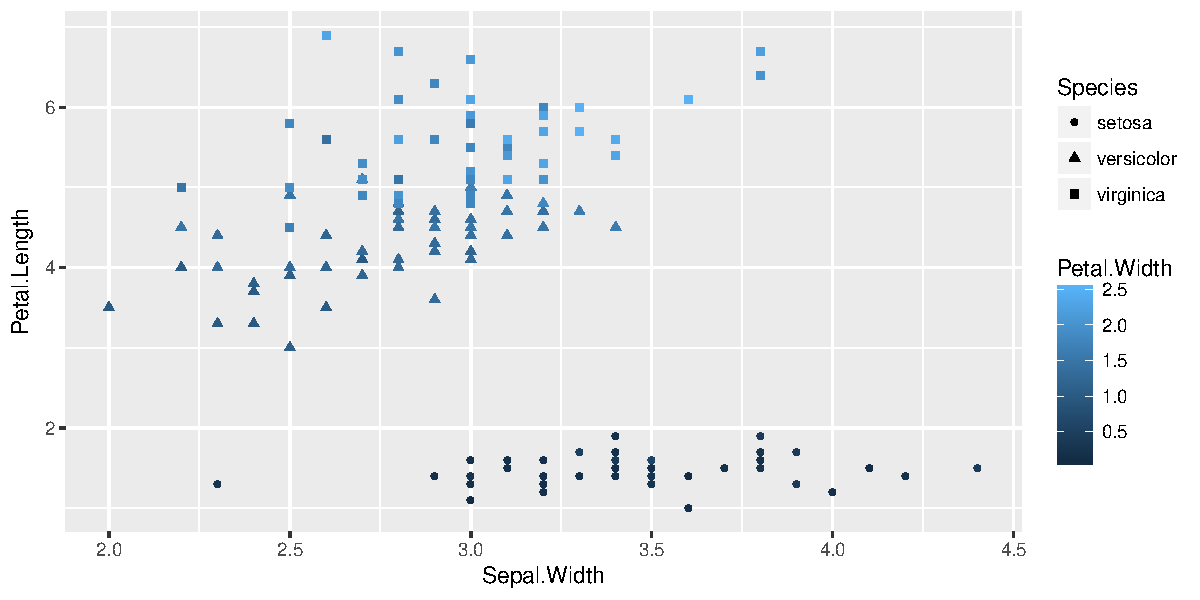
\includegraphics[width=\maxwidth]{figure/unnamed-chunk-3-1} 

\end{knitrout}
\end{frame}

\section{Intro}

\begin{frame}
\frametitle{Plan}
\begin{itemize}
	\item We're going to focus on two things 

	\begin{enumerate}
		\item Theoretical --- control statements and loops

		\item Practical --- applying numpy and scipy to analyze sound 
	\end{enumerate}

	\item What we'll need
	\begin{enumerate}
		\item Python 3 (through IPython)

		\item numpy, scipy, matplotlib, sounddevice

		\item Sound files (in folder "samples") 
	\end{enumerate}

	\item Overview
	\begin{enumerate}
		\item Get the packages we need

		\item Set up editor 

		\item A brief intro to loops

		\item Make one spectrogram

		\item Make a bunch of spectrograms
	\end{enumerate}
\end{itemize}
\end{frame}

\section{Packages}

\begin{frame}[fragile]
\frametitle{Installing sounddevice}
	\begin{itemize}
		\item Why we need each of the following packages is explained later!

		\item We should already have numpy, scipy, and matplotlib installed through Conda

		\item However, we do need to install sounddevice, which will allow us to play sound from a numpy array

		\item To do this using Conda, we type in a generic terminal window... 

		conda list

		\item We notice sounddevice is not on our list, so...

		conda search sounddevice
		
		conda install sounddevice

	\end{itemize}
\end{frame}

\section{Scripts}

\begin{frame}
\frametitle{Editors}
\begin{itemize}
	\item Today, we'll just be writing scripts in Notepad, saving them to disk, and then running them through the IPython terminal 
	\item You'll soon probably want something more fully fledged, more like MATLAB or RStudio
	\begin{enumerate}
		\item Spyder

		\item Eclipse

		\item SublimeText

		\item PyCharm
	\end{enumerate}

	\item Now, let's open up Notepad... 
\end{itemize}
\end{frame}

\begin{frame}
\frametitle{Writing and running a script}
\begin{itemize}
	\item First we write a series of commands in Notepad

	\item Note that Python is sensitive to indentation --- where MATLAB uses "end" and R brackets, Python uses indentation to indicate nested statements and such

	\item Starting with something simple...

\begin{knitrout}
\definecolor{shadecolor}{rgb}{0.969, 0.969, 0.969}\color{fgcolor}\begin{kframe}
\noindent
\ttfamily
\hlstd{}\hlkwa{print}\hlstd{}\hlopt{(}\hlstd{}\hlnum{2}\hlstd{}\hlopt{+}\hlstd{}\hlnum{2}\hlstd{}\hlopt{)}\hlstd{}\hspace*{\fill}
\mbox{}
\normalfont
\end{kframe}
\end{knitrout}

	\item Save this using Notepad to a file called "test.py"

	\item Then, in your terminal, say...
	
	python3 C:/your\_directory\_here/test.py
\end{itemize}
\end{frame}

\section{Loops}

\begin{frame}[fragile]
\frametitle{Our first loop}
\begin{itemize}
	\item Loops in Python have a very easy and powerful syntax

\end{itemize}
\begin{knitrout}
\definecolor{shadecolor}{rgb}{0.969, 0.969, 0.969}\color{fgcolor}\begin{kframe}
\noindent
\ttfamily
\hlstd{}\hlkwa{for\ }\hlstd{i\ }\hlkwa{in\ }\hlstd{}\hlkwb{range}\hlstd{}\hlopt{(}\hlstd{}\hlnum{5}\hlstd{}\hlopt{):}\hspace*{\fill}\\
\hlstd{\ }\hlkwa{print}\hlstd{}\hlopt{(}\hlstd{i}\hlopt{)}\hlstd{}\hspace*{\fill}
\mbox{}
\normalfont

\begin{verbatim}
## 0
## 1
## 2
## 3
## 4
\end{verbatim}
\end{kframe}
\end{knitrout}

\end{frame}

\begin{frame}[fragile]
\frametitle{Loop syntax}
\begin{itemize}
	\item As previously mentioned, Python uses indentation to indicate nesting

	\item If we don't indent at least one line for a loop we'll have problems

	\item I personally like this, I think it promotes more readable code!

\end{itemize}
\begin{knitrout}
\definecolor{shadecolor}{rgb}{0.969, 0.969, 0.969}\color{fgcolor}\begin{kframe}
\noindent
\ttfamily
\hlstd{}\hlkwa{for\ }\hlstd{i\ }\hlkwa{in\ }\hlstd{}\hlkwb{range}\hlstd{}\hlopt{(}\hlstd{}\hlnum{5}\hlstd{}\hlopt{):}\hspace*{\fill}\\
\hlstd{}\hlkwa{print}\hlstd{}\hlopt{(}\hlstd{i}\hlopt{)}\hlstd{}\hspace*{\fill}
\mbox{}
\normalfont

\begin{verbatim}
##   File "<string>", line 2
##     print(i)
##         ^
## IndentationError: expected an indented block
\end{verbatim}
\end{kframe}
\end{knitrout}

\end{frame}

\begin{frame}[fragile]
\frametitle{Looping over other things}
\begin{itemize}
	\item We can loop over a variety of objects

	\item The range() function is for when we want integer sequences, but many things in Python can be used to create a loop (technically, these things are called iterables in Python-lingo)

	\item Lists are iterables...

	\item You can also define your own custom objects to be iterables!

\end{itemize}
\begin{knitrout}
\definecolor{shadecolor}{rgb}{0.969, 0.969, 0.969}\color{fgcolor}\begin{kframe}
\noindent
\ttfamily
\hlstd{x\ }\hlopt{=\ {[}}\hlstd{}\hlnum{1}\hlstd{}\hlopt{,}\hlstd{}\hlnum{4}\hlstd{}\hlopt{,}\hlstd{}\hlnum{9}\hlstd{}\hlopt{,}\hlstd{}\hlnum{16}\hlstd{}\hlopt{,}\hlstd{}\hlnum{25}\hlstd{}\hlopt{{]}}\hspace*{\fill}\\
\hlstd{}\hlkwa{for\ }\hlstd{i\ }\hlkwa{in\ }\hlstd{x}\hlopt{:}\hspace*{\fill}\\
\hlstd{\ }\hlkwa{print}\hlstd{}\hlopt{(}\hlstd{}\hlkwb{str}\hlstd{}\hlopt{(}\hlstd{i}\hlopt{)\ +\ }\hlstd{}\hlkwb{str}\hlstd{}\hlopt{(}\hlstd{x}\hlopt{))}\hlstd{}\hspace*{\fill}
\mbox{}
\normalfont

\begin{verbatim}
## 1[1, 4, 9, 16, 25]
## 4[1, 4, 9, 16, 25]
## 9[1, 4, 9, 16, 25]
## 16[1, 4, 9, 16, 25]
## 25[1, 4, 9, 16, 25]
\end{verbatim}
\end{kframe}
\end{knitrout}

\end{frame}

\begin{frame}[fragile]
\frametitle{Looping over other things}
\begin{itemize}
	\item Strings are also iterables... 

\end{itemize}
\begin{knitrout}
\definecolor{shadecolor}{rgb}{0.969, 0.969, 0.969}\color{fgcolor}\begin{kframe}
\noindent
\ttfamily
\hlstd{}\hlkwa{for\ }\hlstd{i\ }\hlkwa{in\ }\hlstd{}\hlstr{"Hello"}\hlstd{}\hlopt{:}\hspace*{\fill}\\
\hlstd{\ }\hlkwa{print}\hlstd{}\hlopt{(}\hlstd{i}\hlopt{)}\hlstd{}\hspace*{\fill}
\mbox{}
\normalfont

\begin{verbatim}
## H
## e
## l
## l
## o
\end{verbatim}
\end{kframe}
\end{knitrout}
\end{frame}

\begin{frame}[fragile]
\frametitle{Nested loops}
\begin{itemize}
	\item Just like in other languages, we can nest for loops to do more powerful things
\end{itemize}
\begin{knitrout}\tiny
\definecolor{shadecolor}{rgb}{0.969, 0.969, 0.969}\color{fgcolor}\begin{kframe}
\noindent
\ttfamily
\hlstd{bases\ }\hlopt{=\ {[}}\hlstd{}\hlnum{1}\hlstd{}\hlopt{,\ }\hlstd{}\hlnum{2}\hlstd{}\hlopt{,\ }\hlstd{}\hlnum{3}\hlstd{}\hlopt{{]}}\hspace*{\fill}\\
\hlstd{expos\ }\hlopt{=\ {[}}\hlstd{}\hlnum{1}\hlstd{}\hlopt{,\ }\hlstd{}\hlnum{2}\hlstd{}\hlopt{,\ }\hlstd{}\hlnum{3}\hlstd{}\hlopt{,\ }\hlstd{}\hlnum{4}\hlstd{}\hlopt{{]}}\hspace*{\fill}\\
\hlstd{}\hlkwa{for\ }\hlstd{base\ }\hlkwa{in\ }\hlstd{bases}\hlopt{:}\hspace*{\fill}\\
\hlstd{\ }\hlkwa{print}\hlstd{}\hlopt{(}\hlstd{}\hlstr{"Base:"}\hlstd{\ }\hlopt{+\ }\hlstd{}\hlkwb{str}\hlstd{}\hlopt{(}\hlstd{base}\hlopt{))}\hspace*{\fill}\\
\hlstd{\ }\hlkwa{for\ }\hlstd{expo\ }\hlkwa{in\ }\hlstd{expos}\hlopt{:}\hspace*{\fill}\\
\hlstd{}\hlstd{\ \ }\hlstd{}\hlkwa{print}\hlstd{}\hlopt{(}\hlstd{}\hlkwb{str}\hlstd{}\hlopt{(}\hlstd{base}\hlopt{)\ +\ }\hlstd{}\hlstr{"\textasciicircum "}\hlstd{\ }\hlopt{+\ }\hlstd{}\hlkwb{str}\hlstd{}\hlopt{(}\hlstd{expo}\hlopt{)\ +\ }\hlstd{}\hlstr{"="}\hlstd{\ }\hlopt{+\ }\hlstd{}\hlkwb{str}\hlstd{}\hlopt{(}\hlstd{base}\hlopt{{*}{*}}\hlstd{expo}\hlopt{))}\hlstd{}\hspace*{\fill}
\mbox{}
\normalfont

\begin{verbatim}
## Base:1
## 1^1=1
## 1^2=1
## 1^3=1
## 1^4=1
## Base:2
## 2^1=2
## 2^2=4
## 2^3=8
## 2^4=16
## Base:3
## 3^1=3
## 3^2=9
## 3^3=27
## 3^4=81
\end{verbatim}
\end{kframe}
\end{knitrout}
\end{frame}

\begin{frame}[fragile]
\begin{itemize}
	\item Naturally, we can mix loops and other control statements 

\begin{knitrout}\tiny
\definecolor{shadecolor}{rgb}{0.969, 0.969, 0.969}\color{fgcolor}\begin{kframe}
\noindent
\ttfamily
\hlstd{}\hlkwa{for\ }\hlstd{i\ }\hlkwa{in\ }\hlstd{}\hlkwb{range}\hlstd{}\hlopt{(}\hlstd{}\hlnum{10}\hlstd{}\hlopt{):}\hspace*{\fill}\\
\hlstd{\ }\hlkwa{if\ }\hlstd{i\ }\hlopt{$<$\ }\hlstd{}\hlnum{3}\hlstd{}\hlopt{:}\hspace*{\fill}\\
\hlstd{}\hlstd{\ \ }\hlstd{}\hlkwa{print}\hlstd{}\hlopt{(}\hlstd{i}\hlopt{)}\hspace*{\fill}\\
\hlstd{\ }\hlkwa{elif\ }\hlstd{i\ }\hlopt{$>$\ }\hlstd{}\hlnum{3\ }\hlstd{}\hlkwa{and\ }\hlstd{i\ }\hlopt{$<$\ }\hlstd{}\hlnum{6}\hlstd{}\hlopt{:}\hspace*{\fill}\\
\hlstd{}\hlstd{\ \ }\hlstd{}\hlkwa{print}\hlstd{}\hlopt{(}\hlstd{i}\hlopt{{*}}\hlstd{}\hlnum{100}\hlstd{}\hlopt{)}\hspace*{\fill}\\
\hlstd{\ }\hlkwa{elif\ }\hlstd{i\ }\hlopt{==\ }\hlstd{}\hlnum{8}\hlstd{}\hlopt{:}\hspace*{\fill}\\
\hlstd{}\hlstd{\ \ }\hlstd{}\hlkwa{break}\hspace*{\fill}\\
\hlstd{\ }\hlkwa{else}\hlstd{}\hlopt{:}\hspace*{\fill}\\
\hlstd{}\hlstd{\ \ }\hlstd{}\hlkwa{print}\hlstd{}\hlopt{(}\hlstd{}\hlstr{"Hello"}\hlstd{}\hlopt{)}\hlstd{}\hspace*{\fill}
\mbox{}
\normalfont

\begin{verbatim}
## 0
## 1
## 2
## Hello
## 400
## 500
## Hello
## Hello
\end{verbatim}
\end{kframe}
\end{knitrout}
\end{itemize}
\end{frame}

\section{Making a spectrogram}
\begin{frame}[fragile]
\frametitle{Setting up the environment}
\begin{itemize}
	\item First, we need to import the necessary modules
\begin{knitrout}
\definecolor{shadecolor}{rgb}{0.969, 0.969, 0.969}\color{fgcolor}\begin{kframe}
\noindent
\ttfamily
\hlstd{}\hspace*{\fill}\\
\hlkwa{import\ }\hlstd{numpy\ }\hlkwa{as\ }\hlstd{np}\hspace*{\fill}\\
\hlkwa{from\ }\hlstd{scipy}\hlopt{.}\hlstd{io\ }\hlkwa{import\ }\hlstd{wavfile}\hspace*{\fill}\\
\hlkwa{import\ }\hlstd{matplotlib}\hlopt{.}\hlstd{pyplot\ }\hlkwa{as\ }\hlstd{plt}\hspace*{\fill}\\
\hlkwa{import\ }\hlstd{sounddevice\ }\hlkwa{as\ }\hlstd{sd}\hspace*{\fill}\\
\hspace*{\fill}
\mbox{}
\normalfont
\end{kframe}
\end{knitrout}
\end{itemize}

\begin{itemize}
	\item numpy --- provides key matrix and DSP operations

	\item wavfile --- provides read/write to wavfile
	
	\item pyplot --- user-friendly functions and objects for plotting

	\item sounddevice --- playback from numpy arrays
\end{itemize}
\end{frame}

\begin{frame}[fragile]
\frametitle{Game Plan}
\begin{enumerate}
		\item Import one signal

		\item Collect measurements of amplitude in each time frequency bin 

		\item Plot it

		\item Save the plot to file

		\item Loop the above four steps as necessary

		\item Put everything in a script
\end{enumerate}
\end{frame}

\begin{frame}[fragile]
\frametitle{Importing a sound file}
\begin{itemize}
	\item The following pertains specifically to certain types of .wav files
	\item For other file types or unusual .wavs, you may need to do some research!
\begin{knitrout}
\definecolor{shadecolor}{rgb}{0.969, 0.969, 0.969}\color{fgcolor}\begin{kframe}
\noindent
\ttfamily
\hlstd{location\ }\hlopt{=\ }\hlstd{}\hlstr{"/home/daniel/Desktop/samples/m03ae.wav"}\hlstd{}\hspace*{\fill}\\
\hlopt{{[}}\hlstd{fs}\hlopt{,\ }\hlstd{y}\hlopt{{]}\ =\ }\hlstd{wavfile}\hlopt{.}\hlstd{}\hlkwd{read}\hlstd{}\hlopt{(}\hlstd{location}\hlopt{)}\hlstd{}\hspace*{\fill}
\mbox{}
\normalfont
\end{kframe}
\end{knitrout}

	\item This will place the sampled waveform contained in m03ae.wav with sample rate fs into the numpy vector y

	\item We can see what this waveform looks like with ...

\begin{knitrout}
\definecolor{shadecolor}{rgb}{0.969, 0.969, 0.969}\color{fgcolor}\begin{kframe}
\noindent
\ttfamily
\hlstd{y\ }\hlopt{=\ }\hlstd{y}\hlopt{/}\hlstd{np}\hlopt{.}\hlstd{}\hlkwb{max}\hlstd{}\hlopt{(}\hlstd{np}\hlopt{.}\hlstd{}\hlkwb{abs}\hlstd{}\hlopt{(}\hlstd{y}\hlopt{))}\hspace*{\fill}\\
\hlstd{plt}\hlopt{.}\hlstd{}\hlkwd{plot}\hlstd{}\hlopt{(}\hlstd{y}\hlopt{)}\hlstd{}\hspace*{\fill}
\mbox{}
\normalfont
\end{kframe}
\end{knitrout}

	\item And what it sounds like with...

\begin{knitrout}
\definecolor{shadecolor}{rgb}{0.969, 0.969, 0.969}\color{fgcolor}\begin{kframe}
\noindent
\ttfamily
\hlstd{sd}\hlopt{.}\hlstd{}\hlkwd{play}\hlstd{}\hlopt{(}\hlstd{y}\hlopt{,}\hlstd{fs}\hlopt{)}\hlstd{}\hspace*{\fill}
\mbox{}
\normalfont
\end{kframe}
\end{knitrout}
\end{itemize}
\end{frame}

\end{document}

